%En el apendice hay que mostrar los two-dimensional histograms que relacionan las 6 variables que usamos en nuestra selection cuts con las 3 variables angular que se emplean para calcular las polarizaciones. Esto son $6 \times 3 =18$ histogramas. Recuérdese que no importa que el fondo esté correlacionado con el ángulo, sólo importa si lo hace la señal. At preselection Level

%The variable that we want to measure is cos\_X\_reco\_tag; the polarization in the Z-axis. \\
%      cos_S_reco_tag  = TMath::Cos(theta_S);  // helicity. theta_S = WBoostedToTopCM->Angle(LeptonBoostedToWCM->Vect();  theta_S = theta^{*}_l. =  polar angle between the charged lepton momentum in the W-boson rest frme

%      cos_LN_reco_tag = TMath::Cos(theta_LN);// polarization N
%      cos_LT_reco_tag = TMath::Cos(theta_LT);// polarization T
%      cos_X_reco_tag  = TMath::Cos(theta_X);  // alphaP with lepton. Polarization in Z-axis. The most important.
%      cos_W_reco_tag  = TMath::Cos(theta_W);  // alphaP with bquark
%      cos_lx_reco_tag = TMath::Cos(theta_lx); // new polarization angle X. theta_lx = leptonInTopCM.Angle(x); x = y.Cross(S)
%      cos_ly_reco_tag = TMath::Cos(theta_ly); // new polarization angle Y. theta_ly = leptonInTopCM.Angle(y); y = S.Cross(((S.Eta()>0.) ? qipos : qineg));

%   S = SpectatorJetBoostedToTopCM->Vect(); Top quark spin direction
%   q = WBoostedToTopCM->Vect(); W boson momentum in the top quark rest frame
%   l = LeptonBoostedToWCM->Vect(); Charged lepton momentum
%   N = S.Cross(q); Normal axis = \hat{s}_t \times \overrightarrow{q}
%   T = q.Cross(N); Transverse axis = \overrightarrow{q} \times Normal axis
%   theta_LN = l.Angle(N); Relative polar angle between $p_l$ and N
%   theta_LT = l.Angle(T);
%   leptonInTopCM = LeptonBoostedToTopCM->Vect();
%   qipos = incomingquarkBoostedToTopCM_pos.Vect();
%   qineg = incomingquarkBoostedToTopCM_neg.Vect();
%     theta_X = leptonInTopCM.Angle(S); where leptonInTopCM= LeptonBoostedToTopCM->Vect()
%     theta_W = S.Angle(q);

In this appendix, the correlations between the six variables used in our final set of selection cuts ($m_{top}$, $H_T$, $\eta_j$, $\Delta\eta_{j,top}$, $m_{j,top}$ and $m_{l,b}$) and the angular distributions of  the cosines of the angles ($\theta_l$, $LX$, $LY$ and $\theta_l^{*}$) are shown.
It is important that a cut on a variable does not remove signal events from the polarisation distributions, otherwise, that variable is not adequate to be included in the set of cuts. 
The displayed angles are those of Section~\ref{sec:ch02}, with the axis definition of reference~\cite{Aguilar-Saavedra:2014eqa}:
\begin{itemize}
\item[$\cos(\theta_l)$]: Cosine of the top-quark polarisation in the $\hat{z}$-axis. The  $\theta_l$ is the angle between the momentum of the charged lepton in the top-quark reference frame with the top-quark spin direction, $\hat{s}_t$. This direction $\hat{s}_t$ is calculated as the spectator jet momentum boosted to the top-quark reference frame. Figures~\ref{Fig:XA}-\ref{Fig:mlbVScosX}.
%This is the most important 
\item[$\cos(LX)$]: Cosine of the top-quark polarisation in the $\hat{x}$-axis. The angle $LX$ is the one formed by the charged lepton in the top-quark reference frame and the $\hat{x}$ defined in equation~\ref{eq:x-axis}. Figures~\ref{Fig:LXA}-\ref{Fig:mlbVScosLX}.
\item[$\cos(LY)$]: Cosine of the top-quark polarisation in the $\hat{y}$-axis. The angle $LX$ is the one formed by the charged lepton in the top-quark reference frame and the $\hat{y}$ defined in equation~\ref{eq:y-axis}. Figures~\ref{Fig:YA}-\ref{Fig:mlbVScosLY}.
\item[$\cos(\theta_l^{*})$]: Cosine of the $W$-boson helicity. $\theta_l^{*}$ is the angle of the $W$-boson momentum in the top-quark reference frame and the charged lepton in the $W$-boson rest frame. Figures~\ref{Fig:SA}-\ref{Fig:SB}.
\end{itemize}
%The axis are those defined in subsection~\ref{subsec:polobs}, which is the convention of~\cite{Aguilar-Saavedra:2014eqa}.
Figures~\ref{Fig:XA}-\ref{Fig:SB} are generated at preselection level (Table~\ref{Table:PreselectionCuts}).

\begin{figure}[h]
\centering
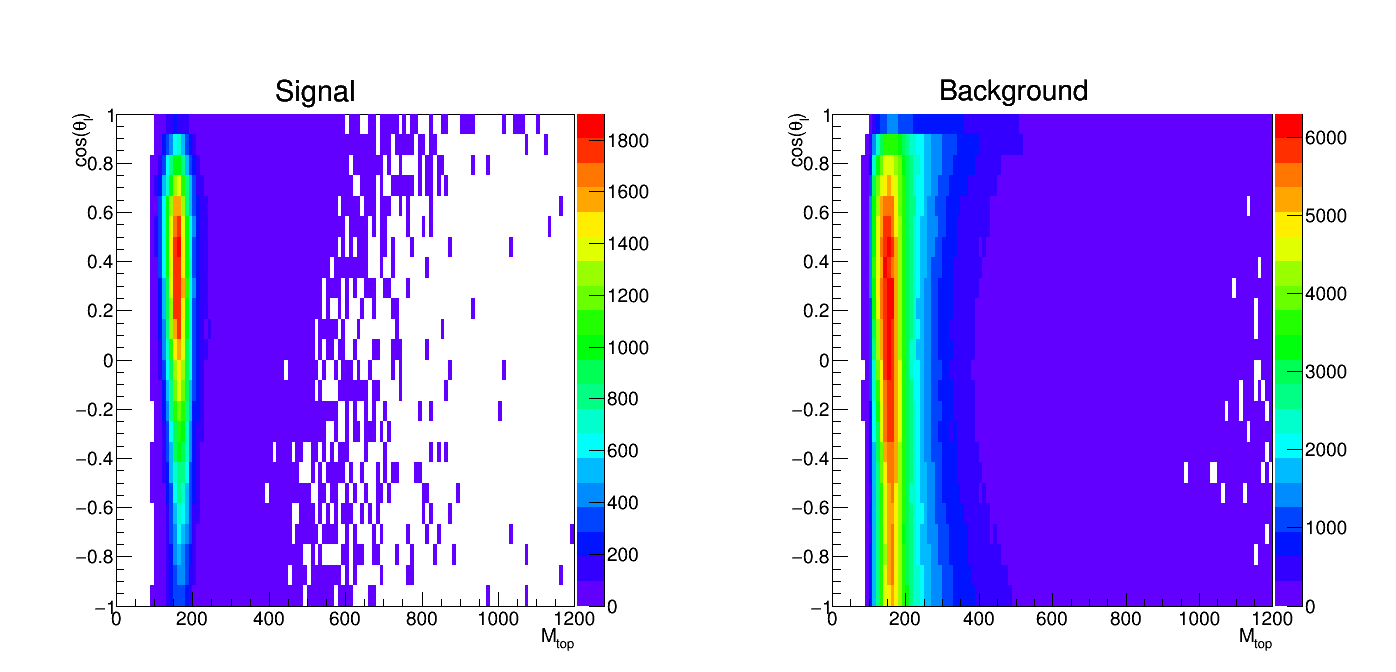
\includegraphics[width=0.9\textwidth]{/afs/ific.uv.es/user/p/pamarag/public/RedaccionTFM/Figuras/Correlation6x3/2d_signal_AND_bkg_PreSelTop_reco_tag_cos_X_kine_topmass_tag.png}
\caption{Two-dimensional distributions of $\cos(\theta_l)$ versus $m_{top}$.}
\label{Fig:XA}
\end{figure}

\begin{figure}[h]
\centering
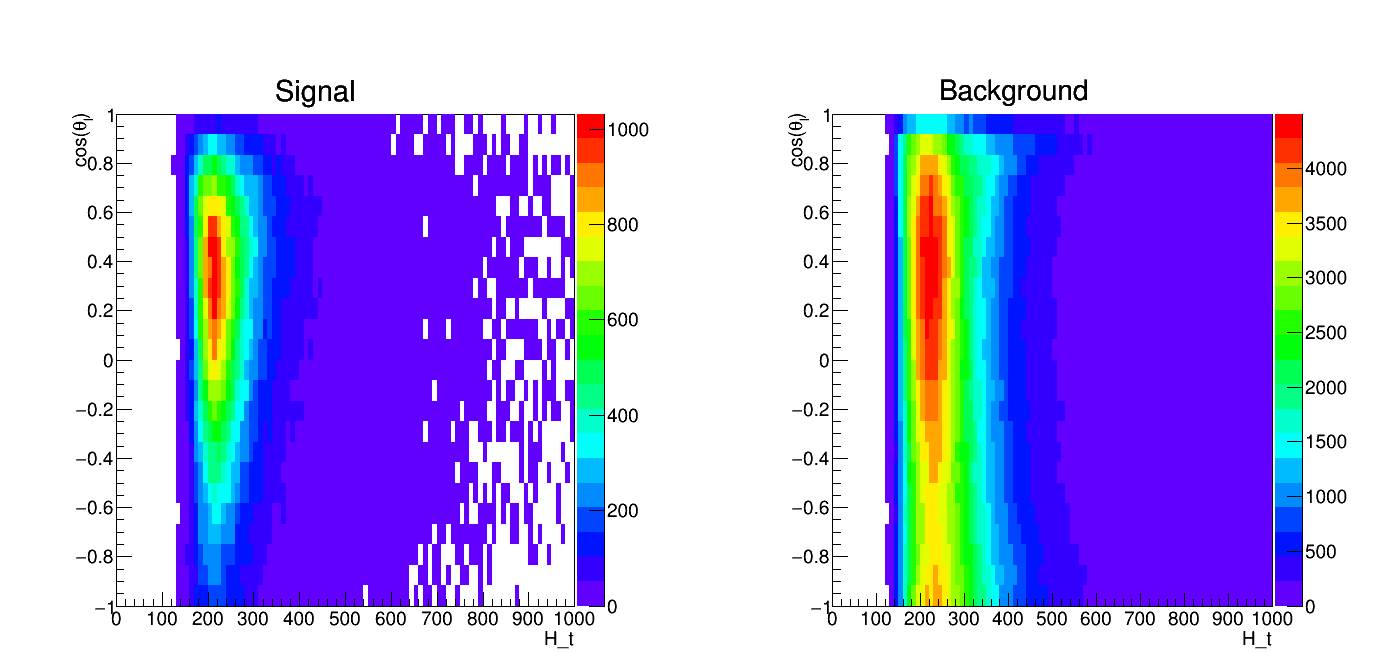
\includegraphics[width=0.9\textwidth]{/afs/ific.uv.es/user/p/pamarag/public/RedaccionTFM/Figuras/Correlation6x3/2d_signal_AND_bkg_PreSelTop_reco_tag_cos_X_kine_ht_tag.png}
\caption{Two-dimensional distributions of $\cos(\theta_l)$ versus $H_T$.}
\end{figure}

\begin{figure}[h]
\centering
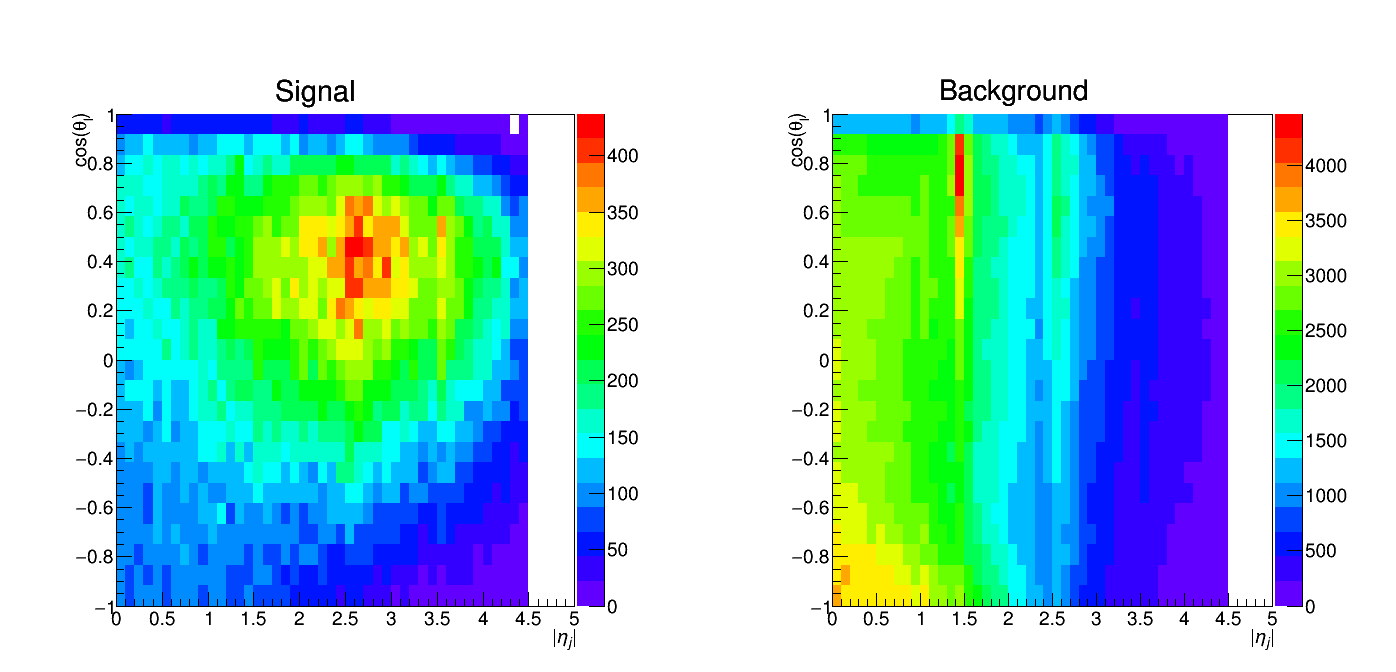
\includegraphics[width=0.9\textwidth]{/afs/ific.uv.es/user/p/pamarag/public/RedaccionTFM/Figuras/Correlation6x3/2d_signal_AND_bkg_PreSelTop_reco_tag_cos_X_kine_eta_lightjet_tag.png}
\caption{Two-dimensional distributions of $\cos(\theta_l)$ versus $\eta_j$.}
\end{figure}

\begin{figure}[h]
\centering
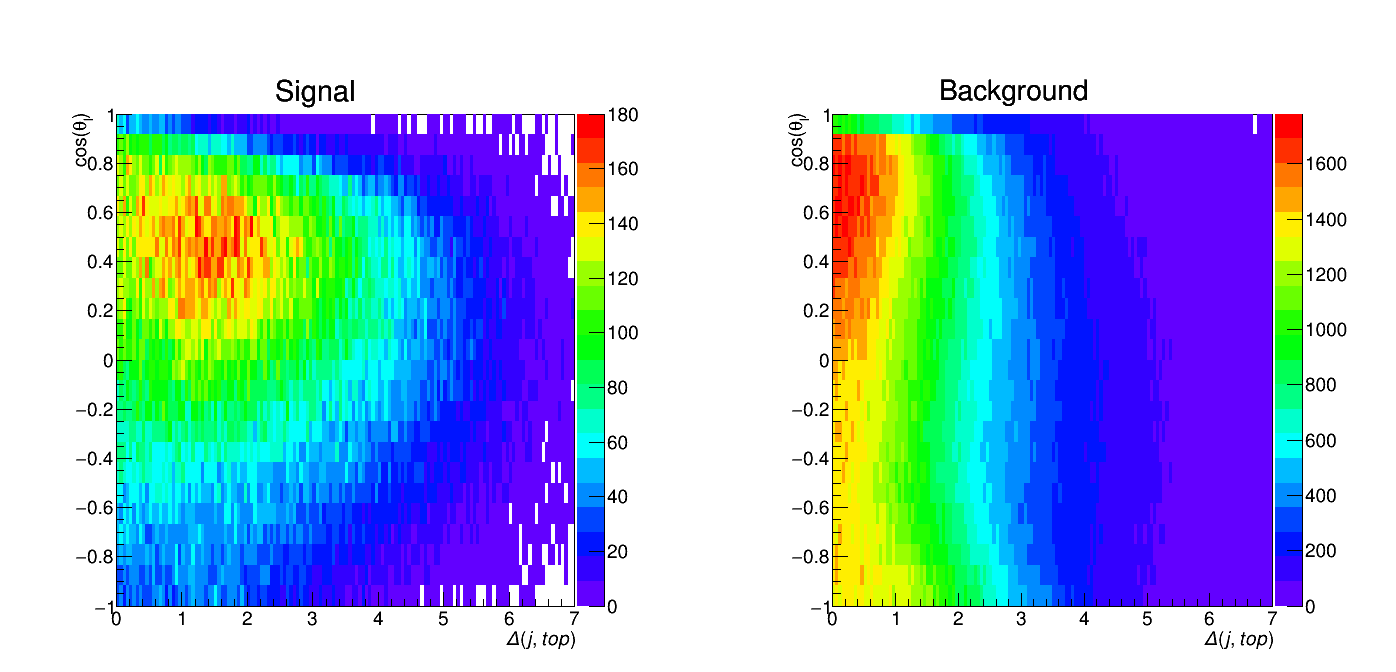
\includegraphics[width=0.9\textwidth]{/afs/ific.uv.es/user/p/pamarag/public/RedaccionTFM/Figuras/Correlation6x3/2d_signal_AND_bkg_PreSelTop_reco_tag_cos_X_dEtajtop.png}
\caption{Two-dimensional distributions of $\cos(\theta_l)$ versus $\Delta\eta_{j,top}$.}
\end{figure}

\begin{figure}[h]
\centering
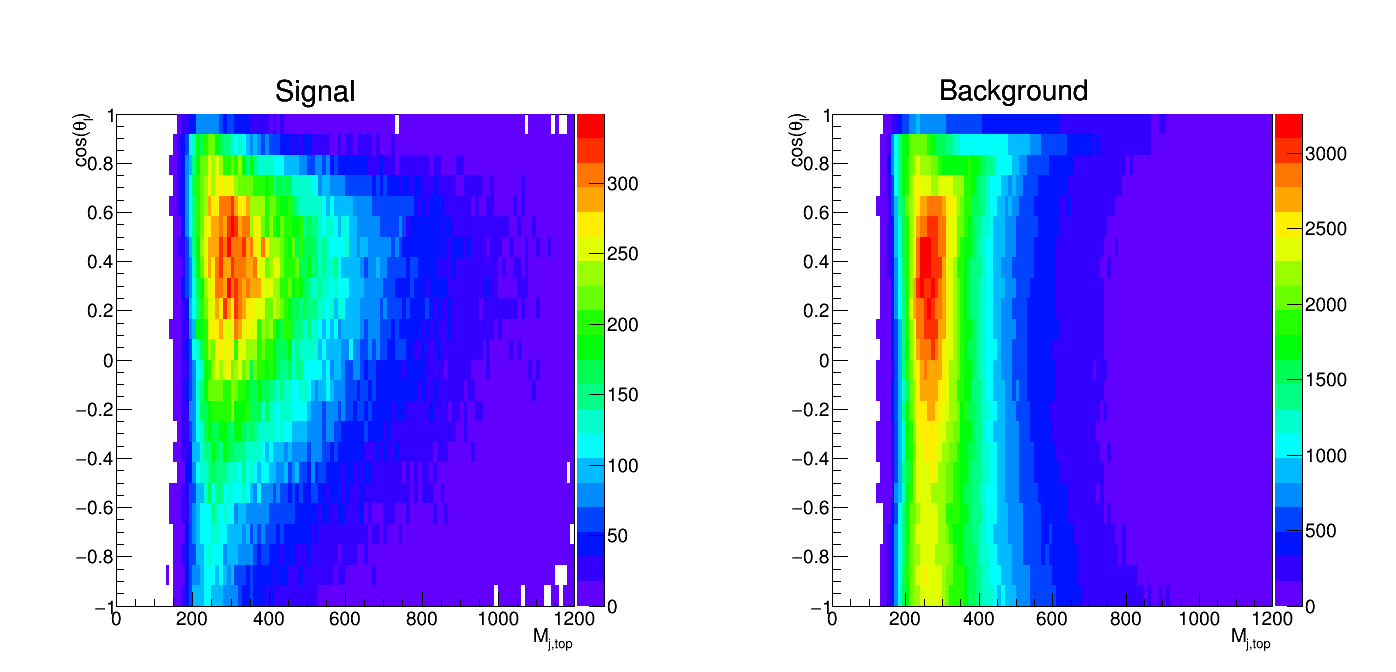
\includegraphics[width=0.9\textwidth]{/afs/ific.uv.es/user/p/pamarag/public/RedaccionTFM/Figuras/Correlation6x3/2d_signal_AND_bkg_PreSelTop_reco_tag_cos_X_Mjtop.png}
\caption{Two-dimensional distributions of $\cos(\theta_l)$ versus $m_{j,top}$.}
\end{figure}

\begin{figure}[h]
\centering
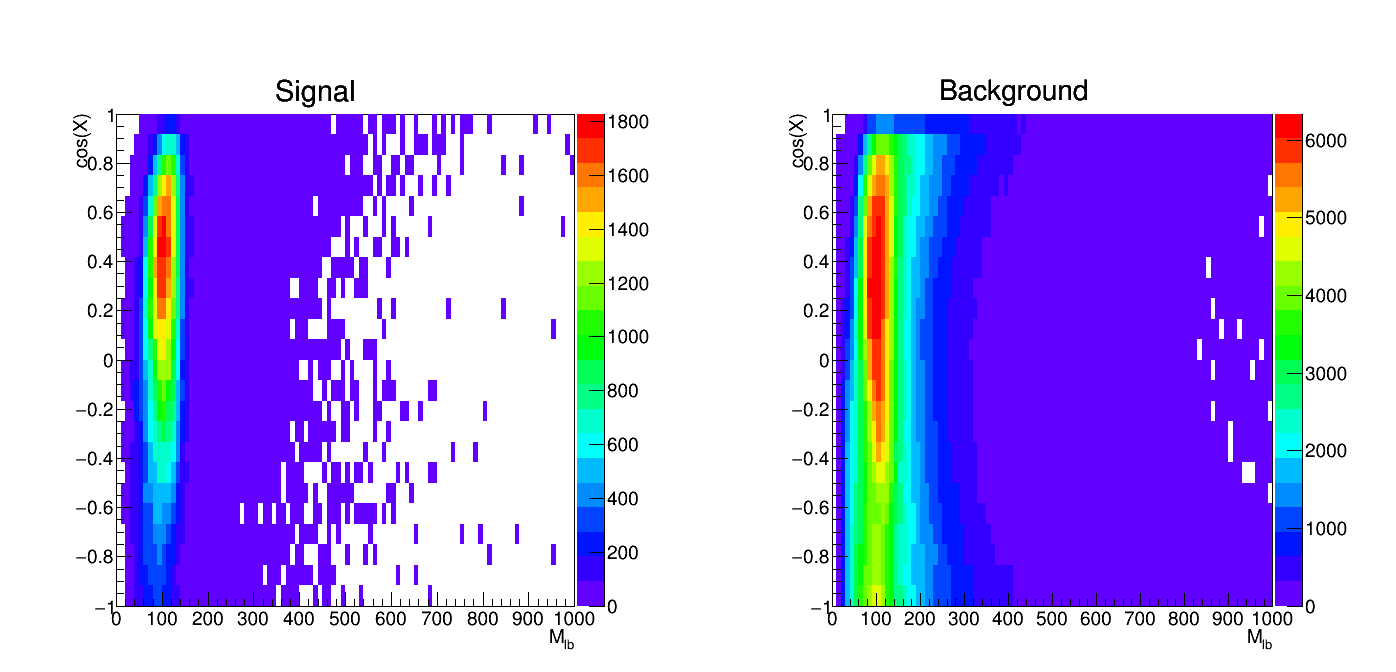
\includegraphics[width=0.95\textwidth]{/afs/ific.uv.es/user/p/pamarag/public/RedaccionTFM/Figuras/2d_signal_AND_bkg_tchannel_reco_tag_cos_X_kine_mlb_tag.png}
\caption{Two-dimensional distributions of $\cos(\theta_l)$ versus $m_{l,b}$.}
\label{Fig:mlbVScosX}
\end{figure}

\begin{figure}[h]
\centering
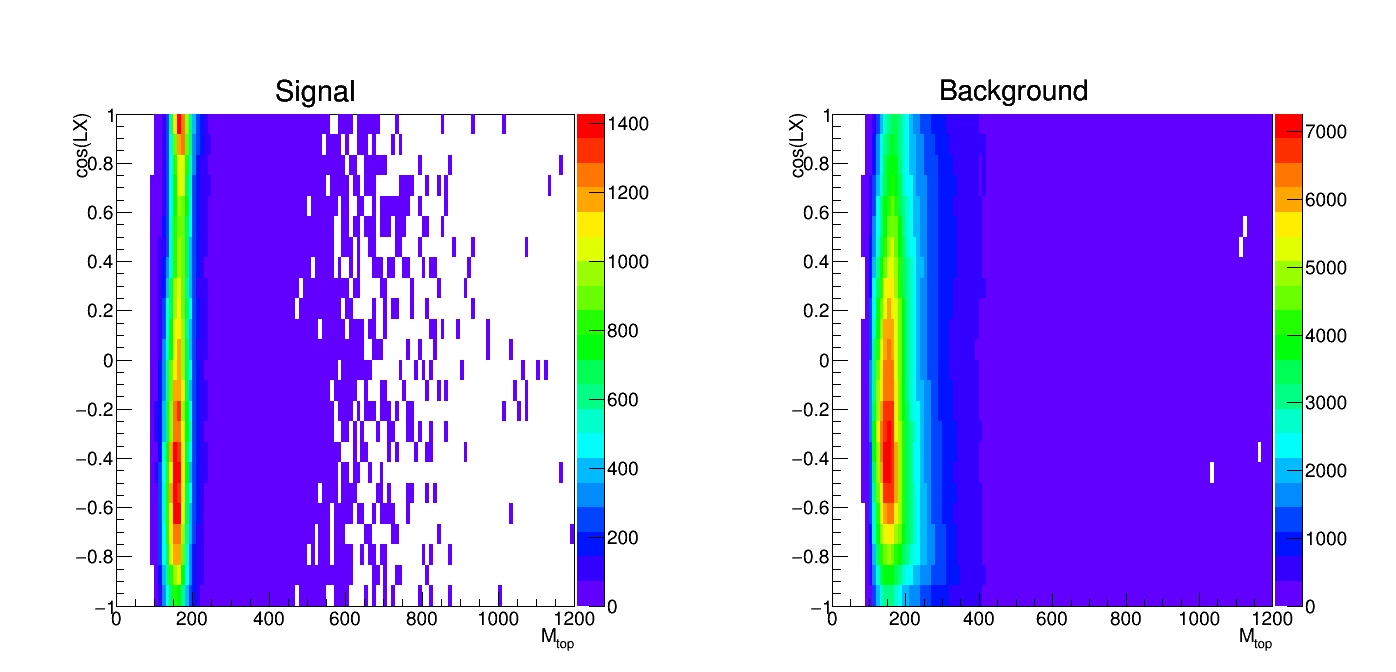
\includegraphics[width=0.9\textwidth]{/afs/ific.uv.es/user/p/pamarag/public/RedaccionTFM/Figuras/Correlation6x3/2d_signal_AND_bkg_PreSelTop_reco_tag_cos_lx_kine_topmass_tag.png}
\caption{Two-dimensional distributions of $\cos(LX)$ versus $m_{top}$.}
\label{Fig:LXA}
\end{figure}

\begin{figure}[h]
\centering
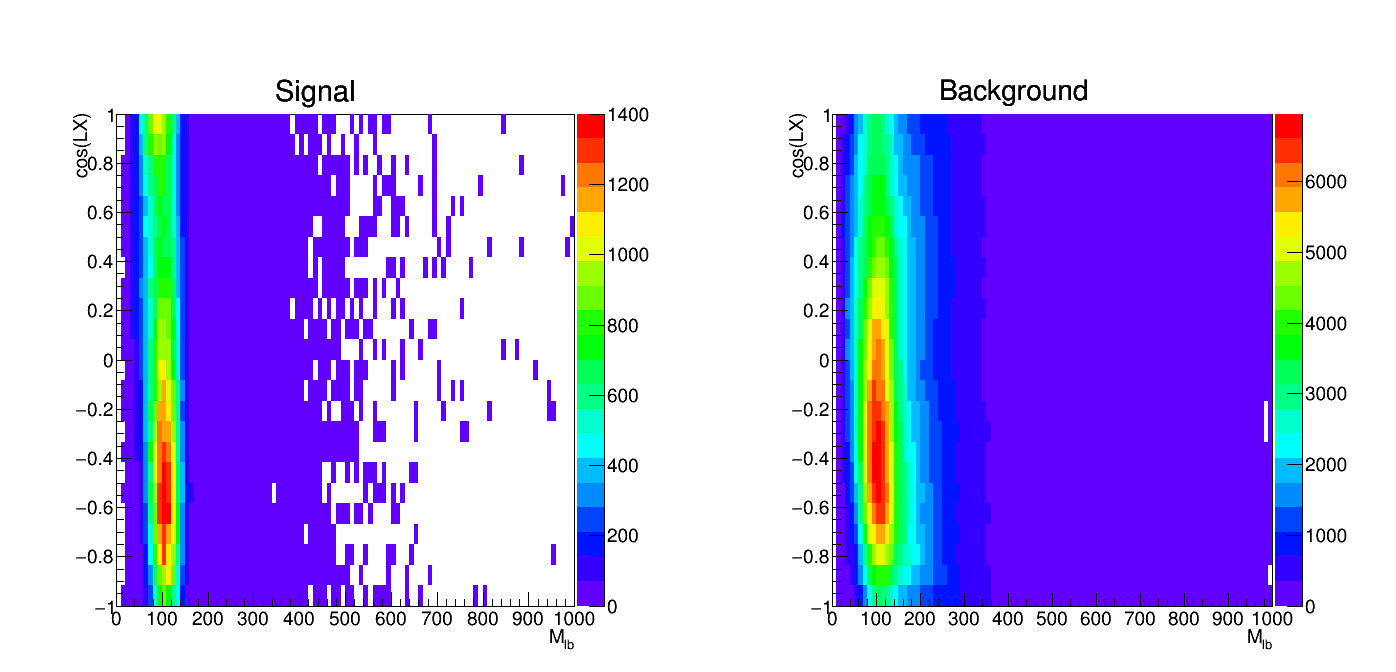
\includegraphics[width=0.9\textwidth]{/afs/ific.uv.es/user/p/pamarag/public/RedaccionTFM/Figuras/Correlation6x3/2d_signal_AND_bkg_PreSelTop_reco_tag_cos_lx_kine_mlb_tag.png}
\caption{Two-dimensional distributions of $\cos(LX)$ versus $H_T$.}
\end{figure}


\begin{figure}[h]
\centering
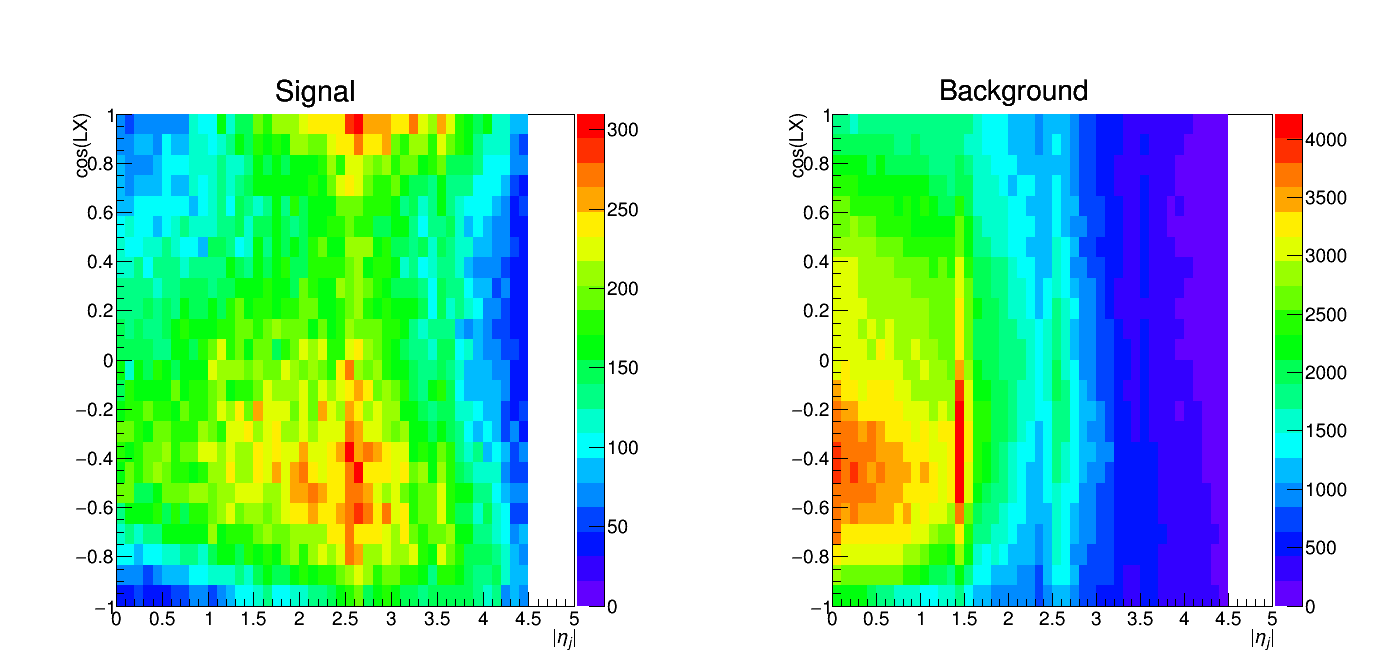
\includegraphics[width=0.9\textwidth]{/afs/ific.uv.es/user/p/pamarag/public/RedaccionTFM/Figuras/Correlation6x3/2d_signal_AND_bkg_PreSelTop_reco_tag_cos_lx_kine_eta_lightjet_tag.png}
\caption{Two-dimensional distributions of $\cos(LX)$ versus $\eta_{j}$.}
\end{figure}

\begin{figure}[h]
\centering
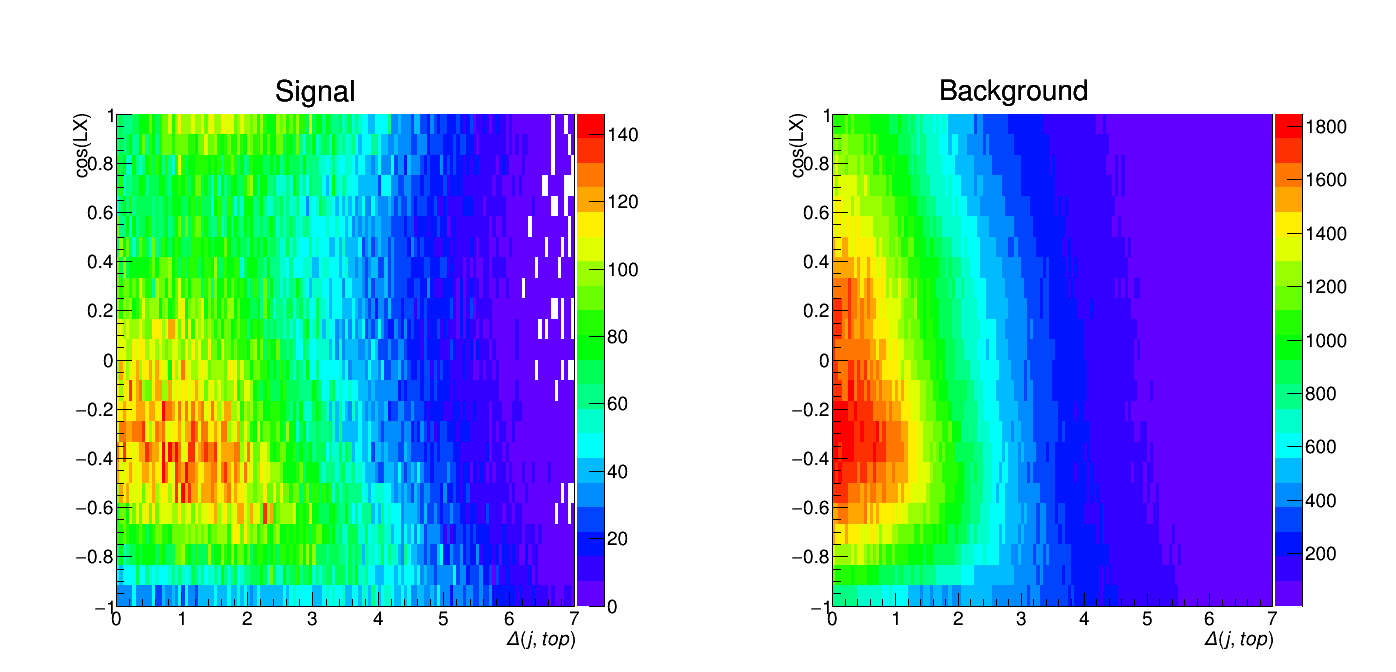
\includegraphics[width=0.9\textwidth]{/afs/ific.uv.es/user/p/pamarag/public/RedaccionTFM/Figuras/Correlation6x3/2d_signal_AND_bkg_PreSelTop_reco_tag_cos_lx_dEtajtop.png}
\caption{Two-dimensional distributions of $\cos(LX)$ versus $\Delta\eta_{j,top}$.}
\end{figure}

\newpage

\begin{figure}[h]
\centering
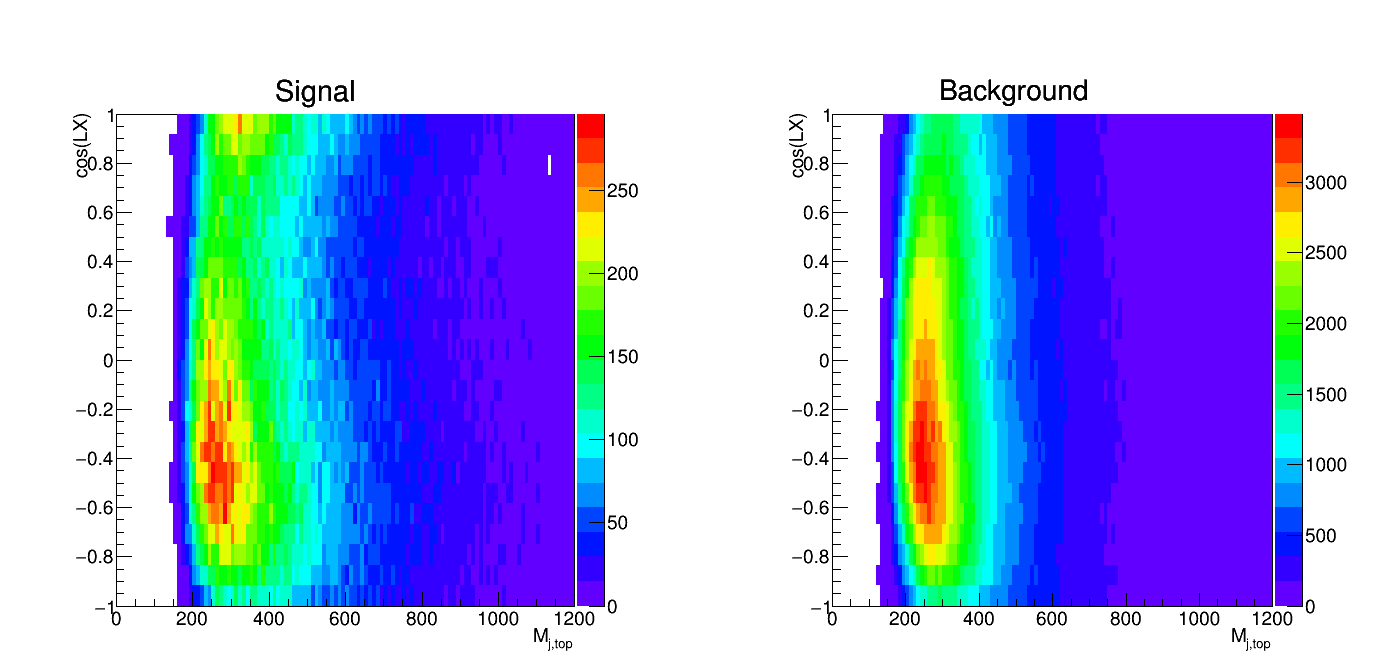
\includegraphics[width=0.9\textwidth]{/afs/ific.uv.es/user/p/pamarag/public/RedaccionTFM/Figuras/Correlation6x3/2d_signal_AND_bkg_PreSelTop_reco_tag_cos_lx_Mjtop.png}
\caption{Two-dimensional distributions of $\cos(LX)$ versus $m_{j,top}$.}
\end{figure}

%\clearpage

\begin{figure}[h]
\centering
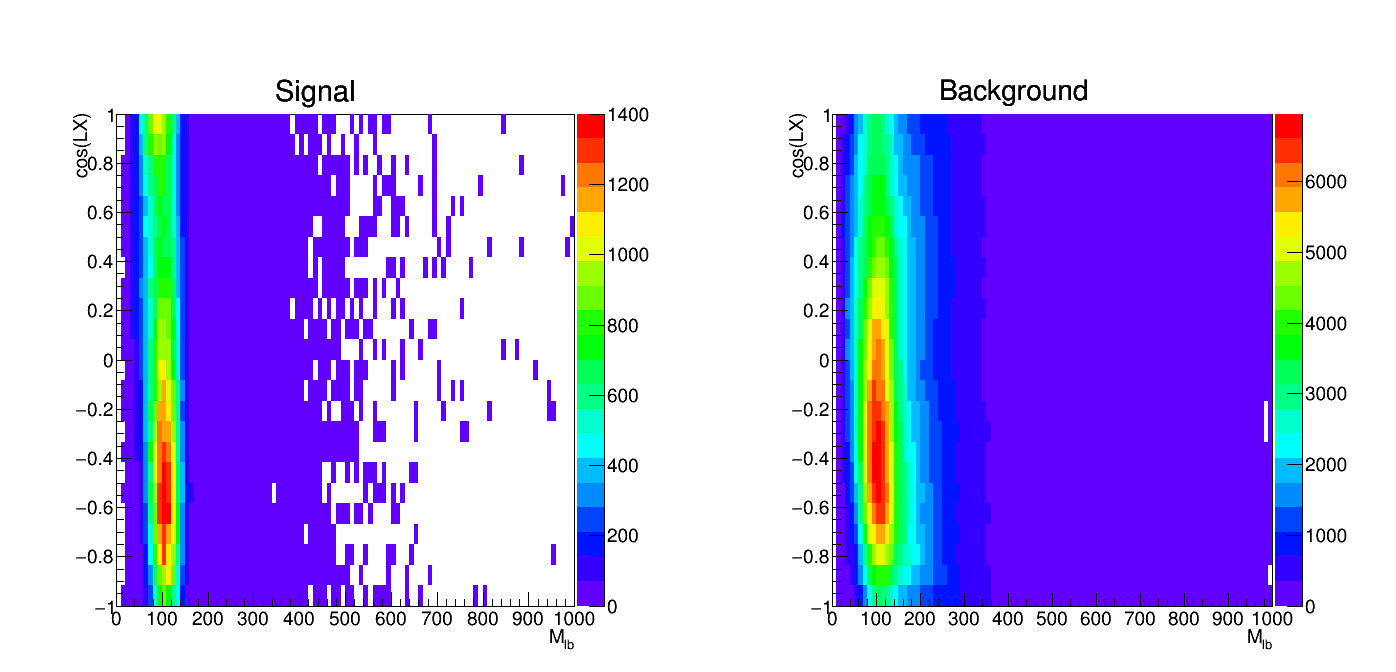
\includegraphics[width=0.9\textwidth]{/afs/ific.uv.es/user/p/pamarag/public/RedaccionTFM/Figuras/Correlation6x3/2d_signal_AND_bkg_PreSelTop_reco_tag_cos_lx_kine_mlb_tag.png}
\caption{Two-dimensional distributions of $\cos(LX)$ versus $m_{l,b}$.}
\label{Fig:mlbVScosLX}
\end{figure}

%%%%
\begin{figure}[h]
\centering
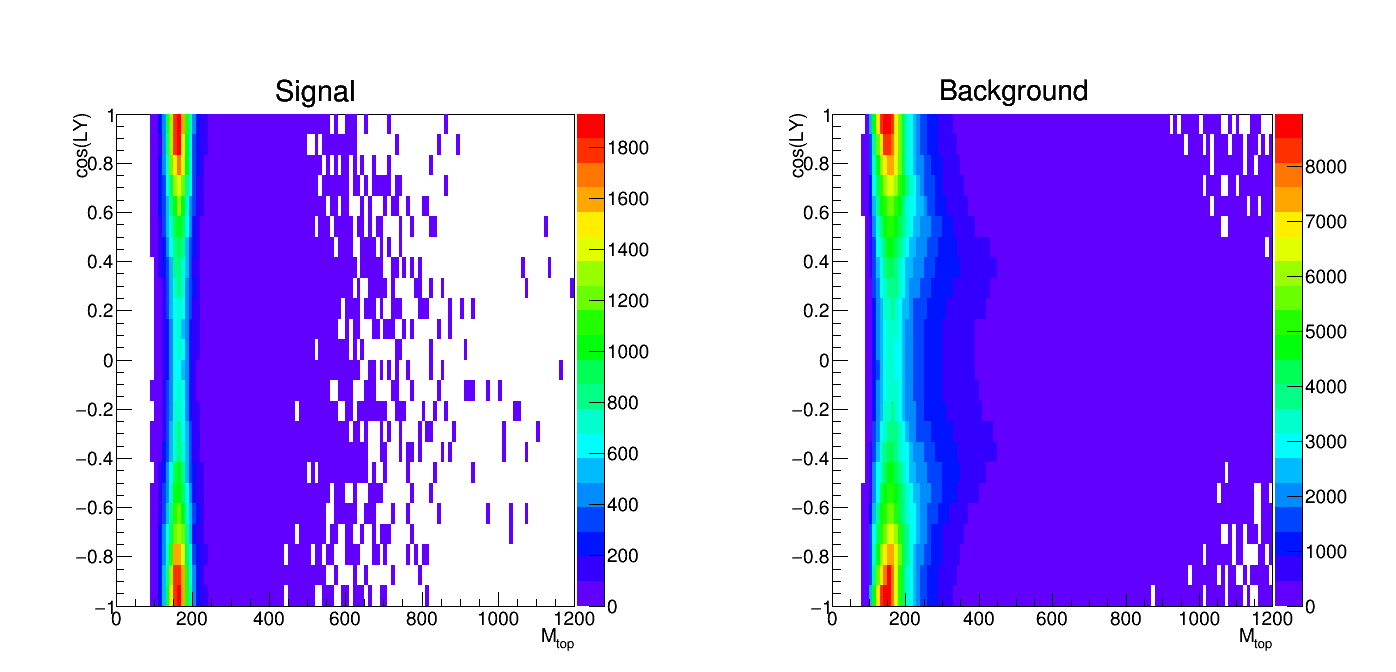
\includegraphics[width=0.9\textwidth]{/afs/ific.uv.es/user/p/pamarag/public/RedaccionTFM/Figuras/Correlation6x3/2d_signal_AND_bkg_PreSelTop_reco_tag_cos_ly_kine_topmass_tag.png}
\caption{Two-dimensional distributions of $\cos(LY)$ versus $m_{top}$.}
\label{Fig:YA}
\end{figure}


\begin{figure}[h]
\centering
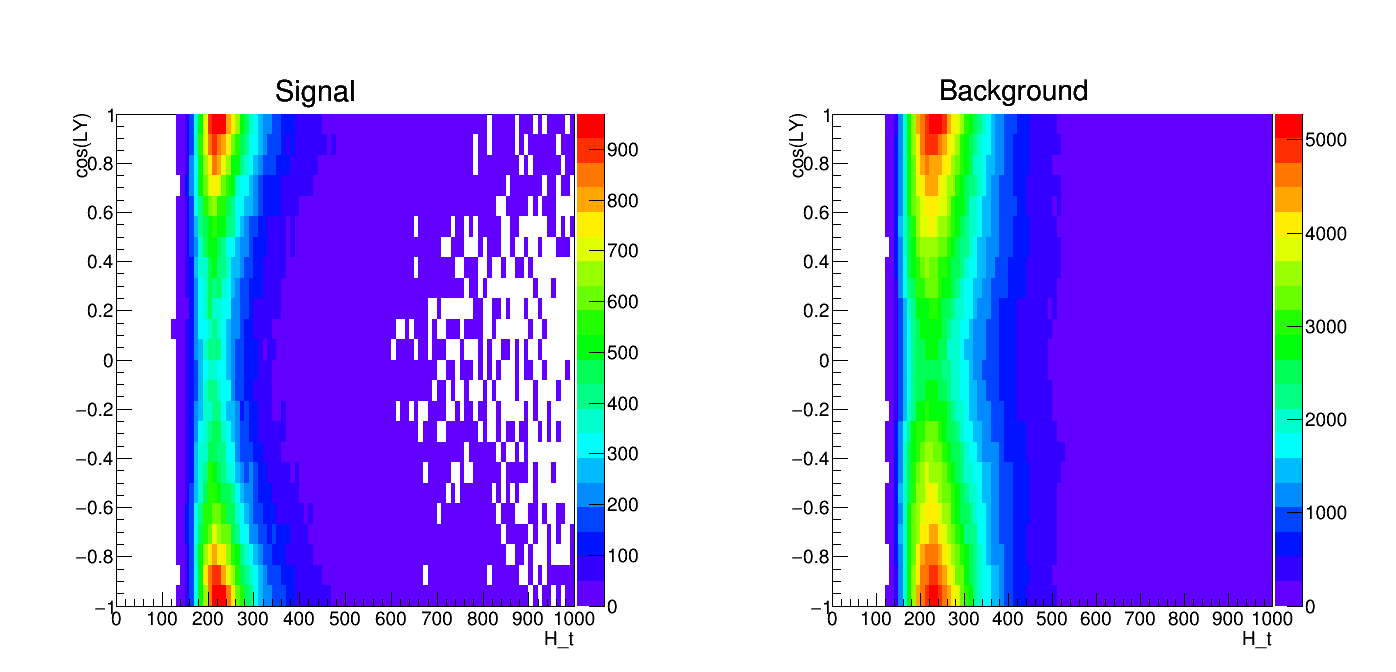
\includegraphics[width=0.9\textwidth]{/afs/ific.uv.es/user/p/pamarag/public/RedaccionTFM/Figuras/Correlation6x3/2d_signal_AND_bkg_PreSelTop_reco_tag_cos_ly_kine_ht_tag.png}
\caption{Two-dimensional distributions of $\cos(LY)$ versus $H_T$.}
\end{figure}


\begin{figure}[h]
\centering
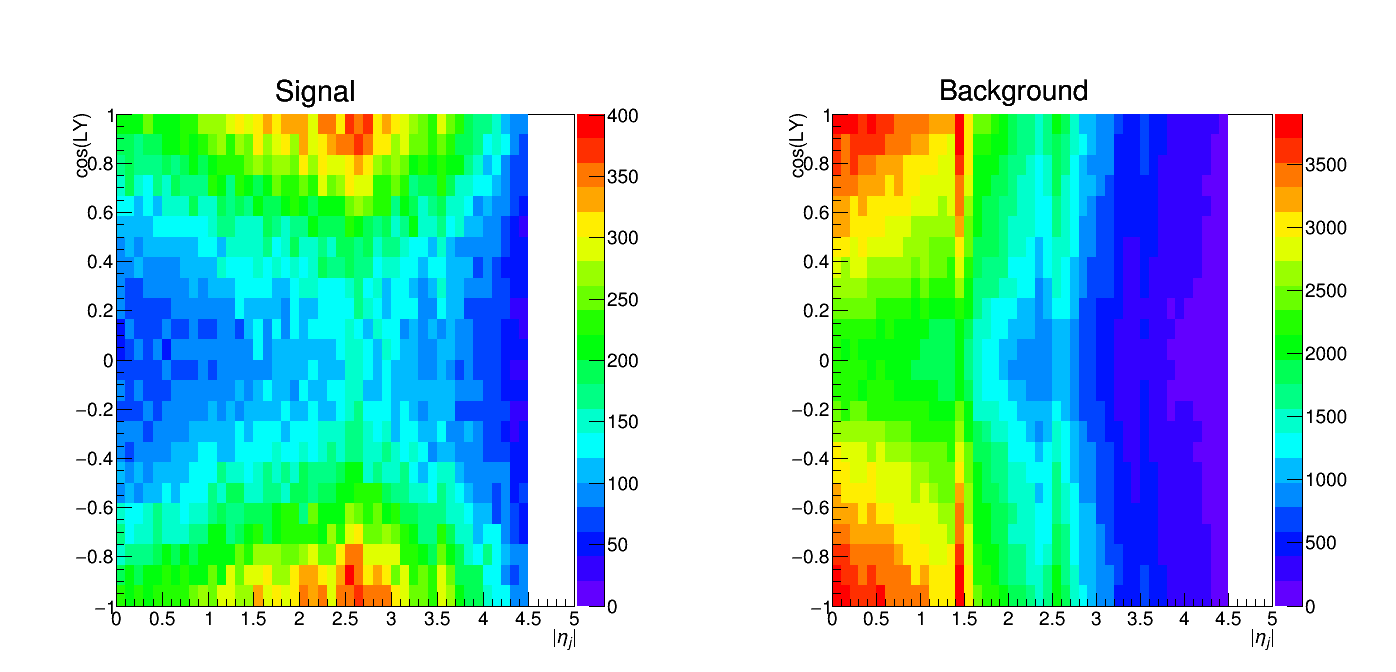
\includegraphics[width=0.9\textwidth]{/afs/ific.uv.es/user/p/pamarag/public/RedaccionTFM/Figuras/Correlation6x3/2d_signal_AND_bkg_PreSelTop_reco_tag_cos_ly_kine_eta_lightjet_tag.png}
\caption{Two-dimensional distributions of $\cos(LY)$ versus $\eta_{j}$.}
\end{figure}

\begin{figure}[h]
\centering
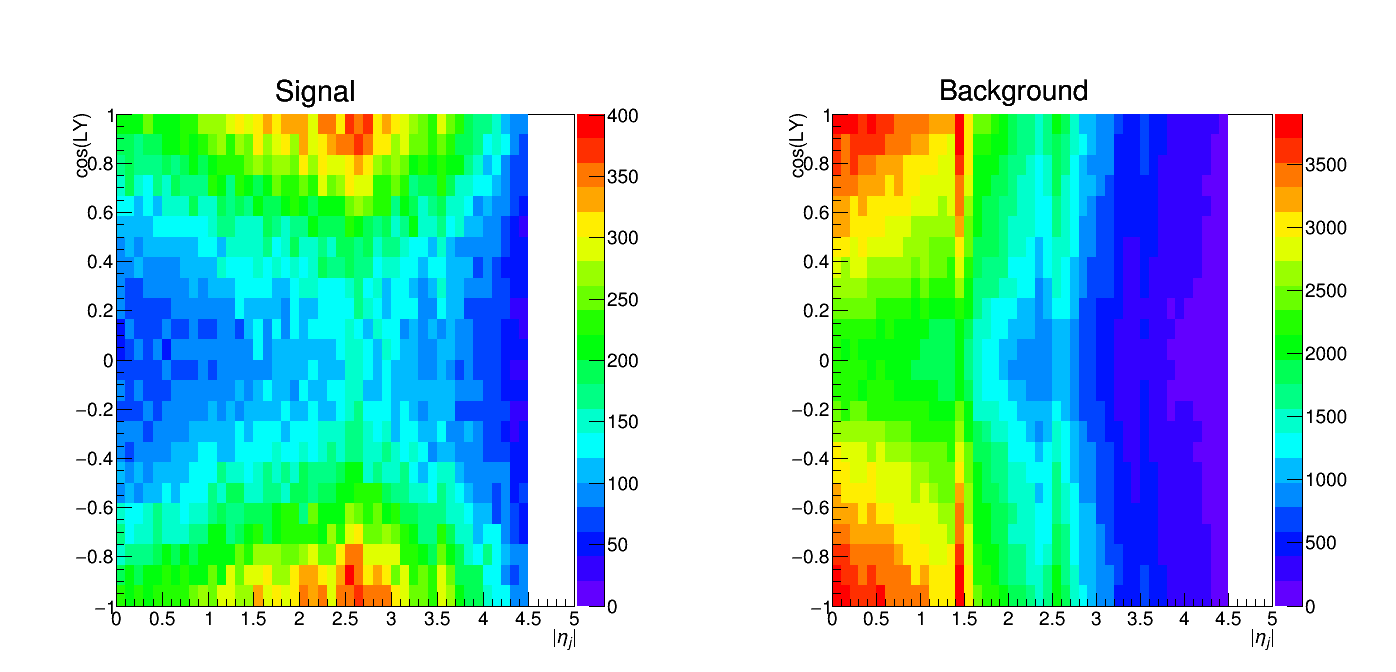
\includegraphics[width=0.9\textwidth]{/afs/ific.uv.es/user/p/pamarag/public/RedaccionTFM/Figuras/Correlation6x3/2d_signal_AND_bkg_PreSelTop_reco_tag_cos_ly_kine_eta_lightjet_tag.png}
\caption{Two-dimensional distributions of $\cos(LY)$ versus $\Delta\eta_{j,top}$.}
\end{figure}

\begin{figure}[h]
\centering
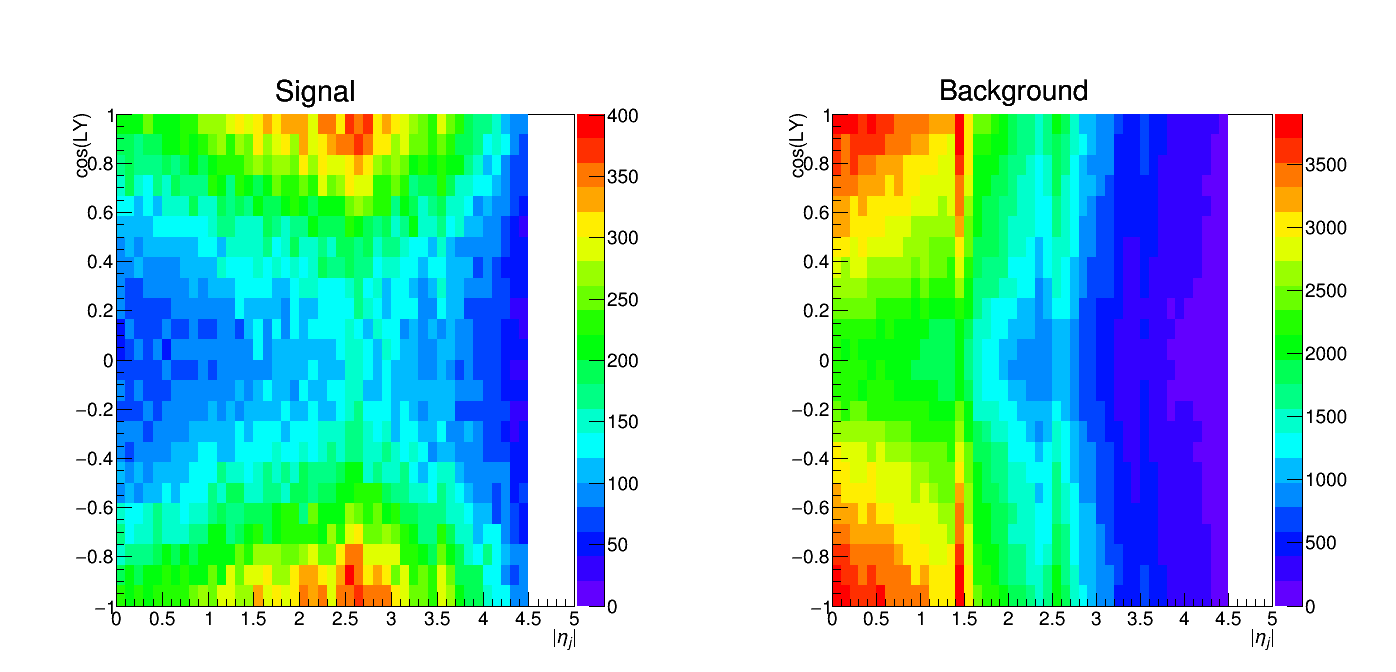
\includegraphics[width=0.9\textwidth]{/afs/ific.uv.es/user/p/pamarag/public/RedaccionTFM/Figuras/Correlation6x3/2d_signal_AND_bkg_PreSelTop_reco_tag_cos_ly_kine_eta_lightjet_tag.png}
\caption{Two-dimensional distributions of $\cos(LY)$ versus $m_{j,top}$.}
\end{figure}


\begin{figure}[h]
\centering
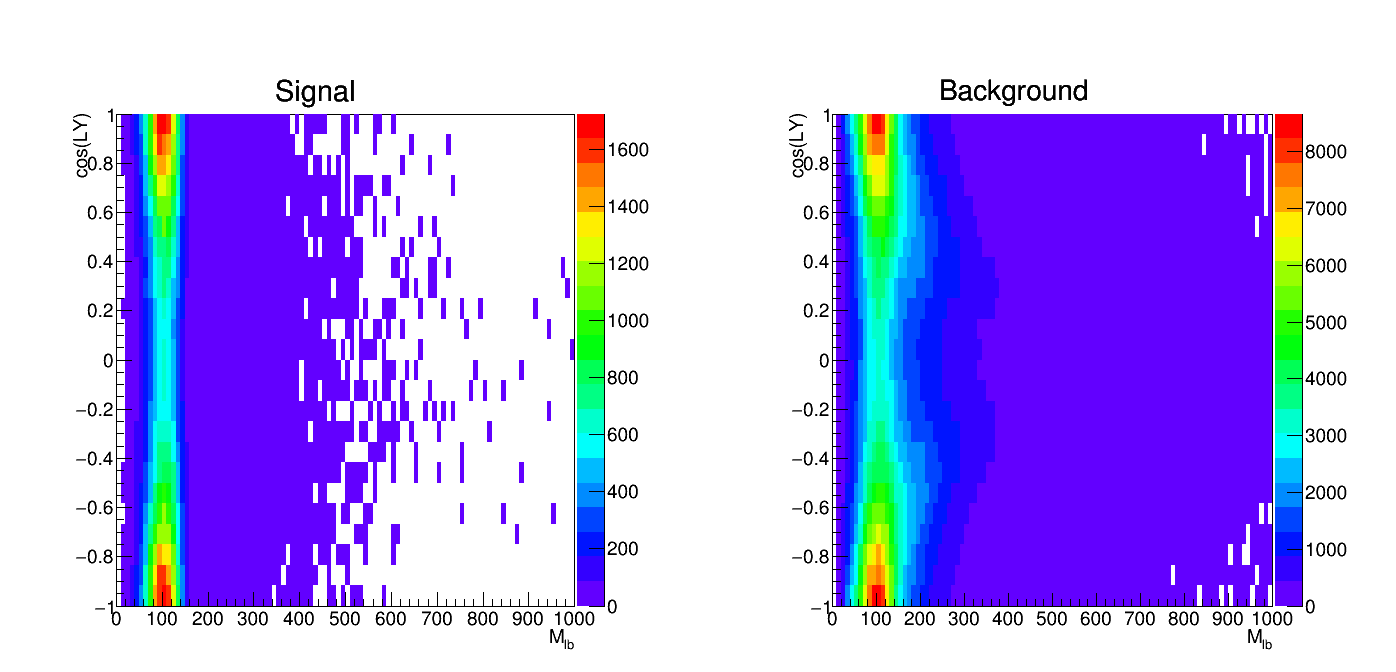
\includegraphics[width=0.9\textwidth]{/afs/ific.uv.es/user/p/pamarag/public/RedaccionTFM/Figuras/Correlation6x3/2d_signal_AND_bkg_PreSelTop_reco_tag_cos_ly_kine_mlb_tag.png}
\caption{Two-dimensional distributions of $\cos(LY)$ versus $m_{l,b}$.}
\label{Fig:mlbVScosLY}
\end{figure}


%%%%%%%%%%%%%%%
\begin{figure}[h]
\centering
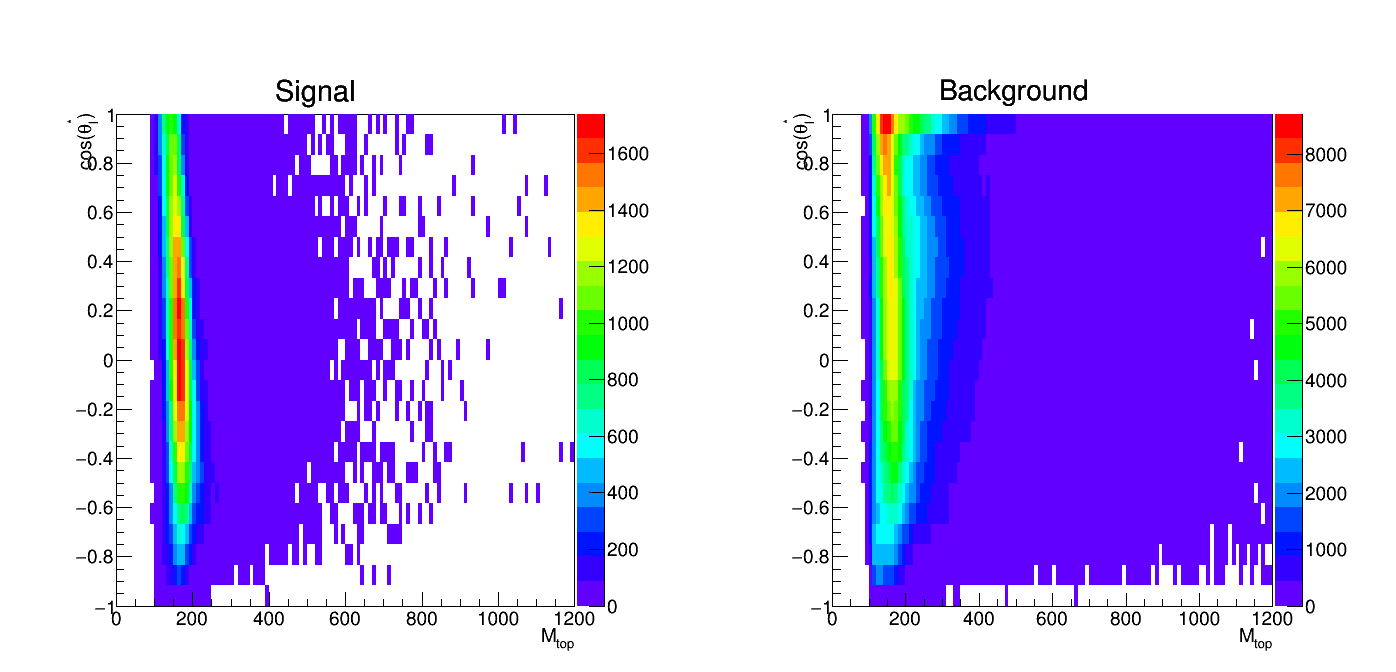
\includegraphics[width=0.9\textwidth]{/afs/ific.uv.es/user/p/pamarag/public/RedaccionTFM/Figuras/Correlation6x3/2d_signal_AND_bkg_PreSelTop_reco_tag_cos_S_kine_topmass_tag.png}
\caption{Two-dimensional distributions of $\cos(\theta_l^{*})$ versus $m_{top}$.}
\label{Fig:SA}
\end{figure}


\clearpage
\vspace*{1cm}
\begin{figure}[h]
\centering
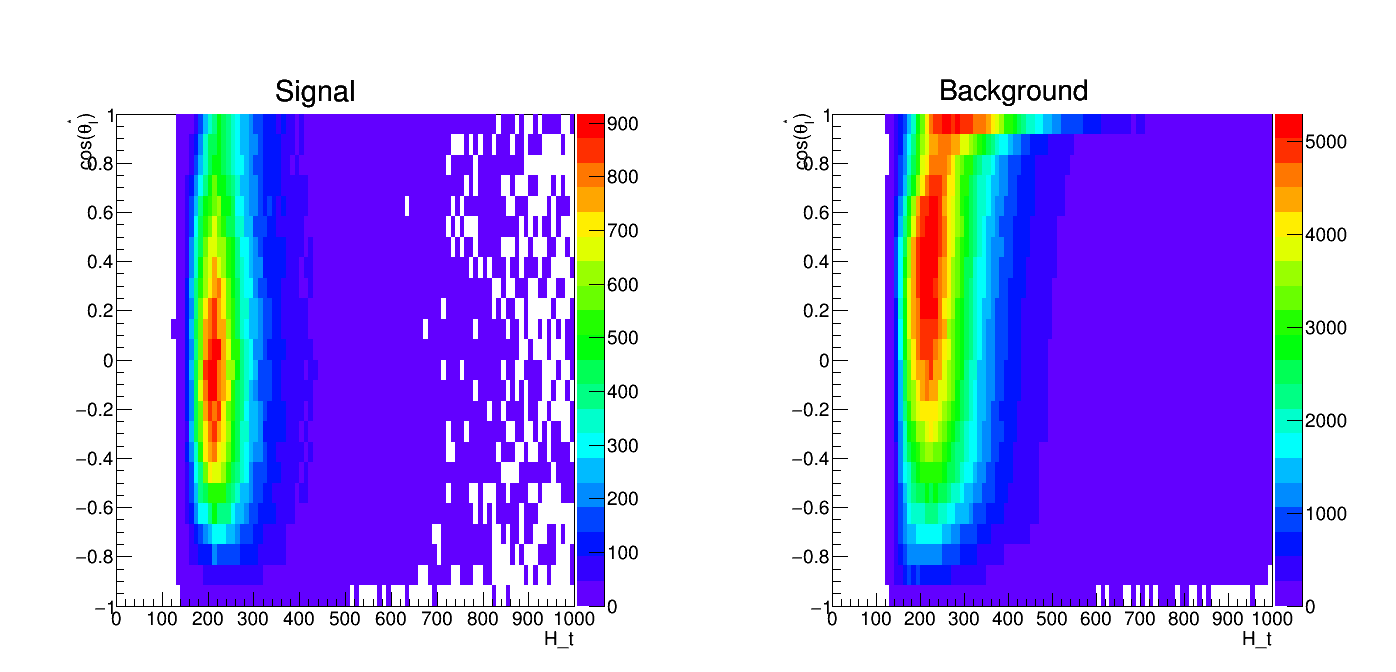
\includegraphics[width=0.9\textwidth]{/afs/ific.uv.es/user/p/pamarag/public/RedaccionTFM/Figuras/Correlation6x3/2d_signal_AND_bkg_PreSelTop_reco_tag_cos_S_kine_ht_tag.png}
\caption{Two-dimensional distributions of $\cos(\theta_l^{*})$ versus $H_T$.}
\end{figure}

\vspace*{5cm}

\begin{figure}[h]
\centering
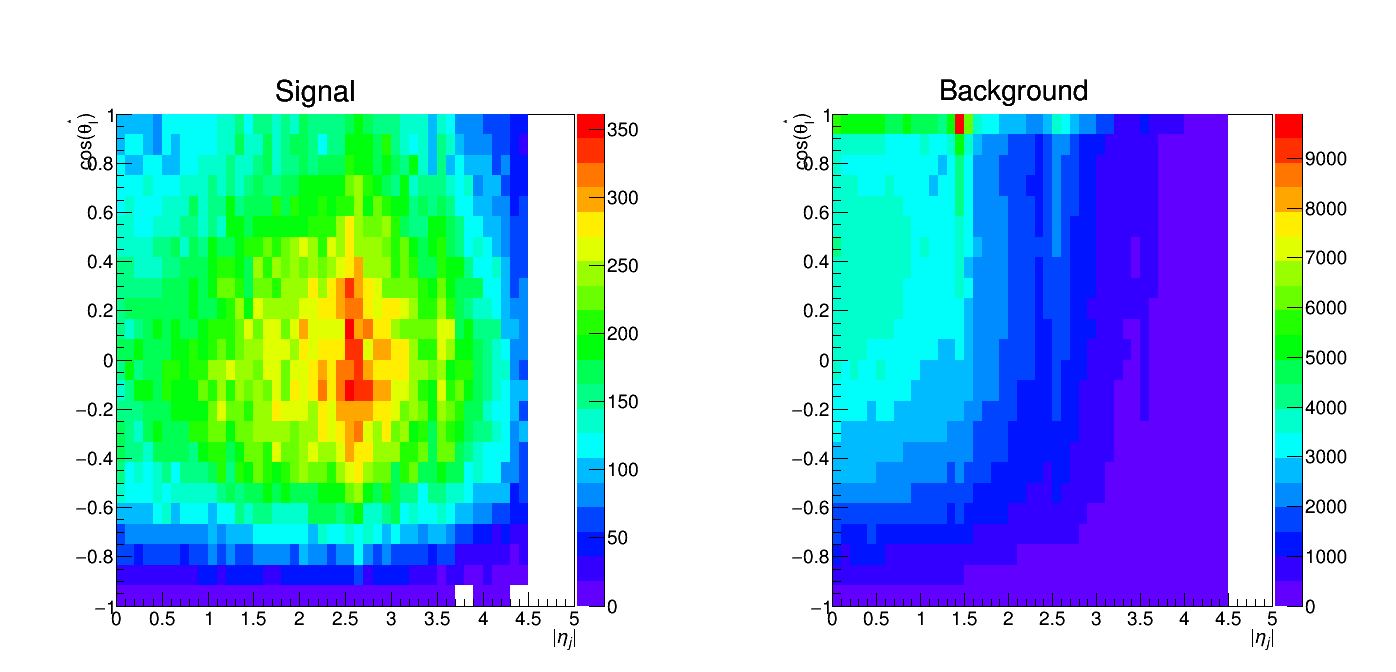
\includegraphics[width=0.9\textwidth]{/afs/ific.uv.es/user/p/pamarag/public/RedaccionTFM/Figuras/Correlation6x3/2d_signal_AND_bkg_PreSelTop_reco_tag_cos_S_kine_eta_lightjet_tag.png}
\caption{Two-dimensional distributions of $\cos(\theta_l^{*})$ versus $\eta_j$.}
\end{figure}

\begin{figure}[h]
\centering
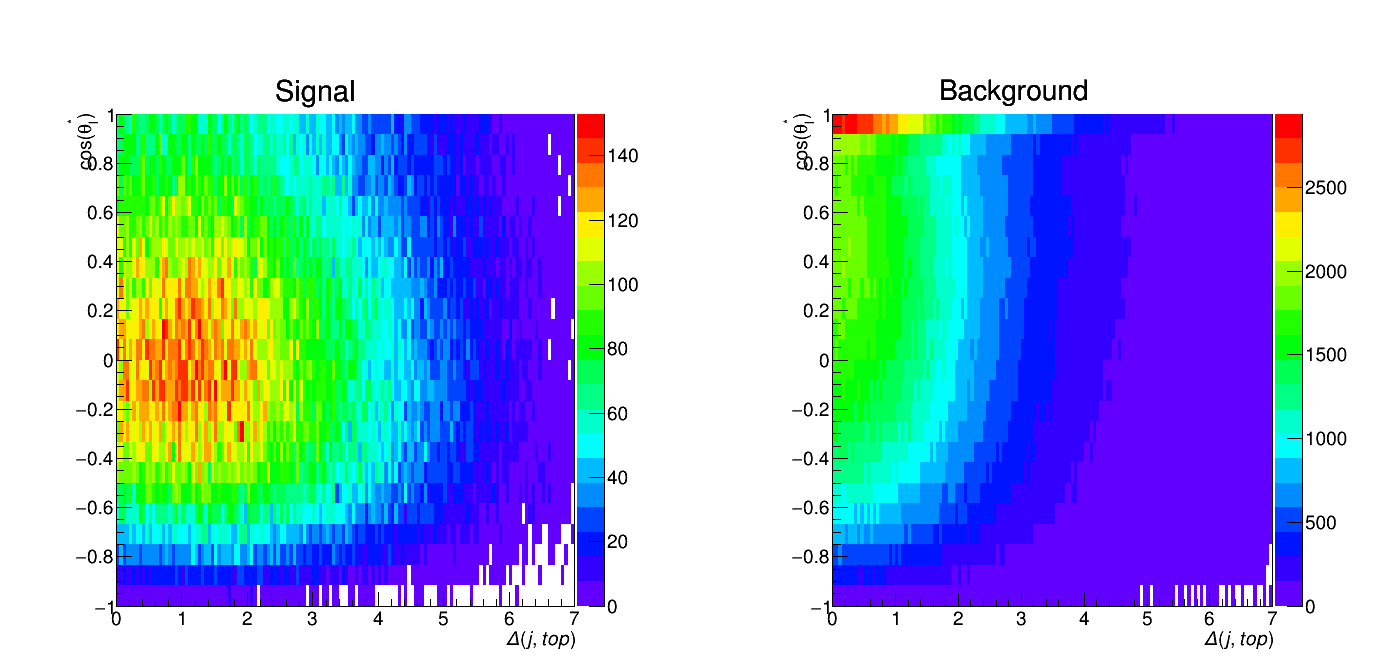
\includegraphics[width=0.9\textwidth]{/afs/ific.uv.es/user/p/pamarag/public/RedaccionTFM/Figuras/Correlation6x3/2d_signal_AND_bkg_PreSelTop_reco_tag_cos_S_dEtajtop.png}
\caption{Two-dimensional distributions of $\cos(\theta_l^{*})$ versus $\Delta\eta_{j,top}$.}
\end{figure}

\begin{figure}[h]
\centering
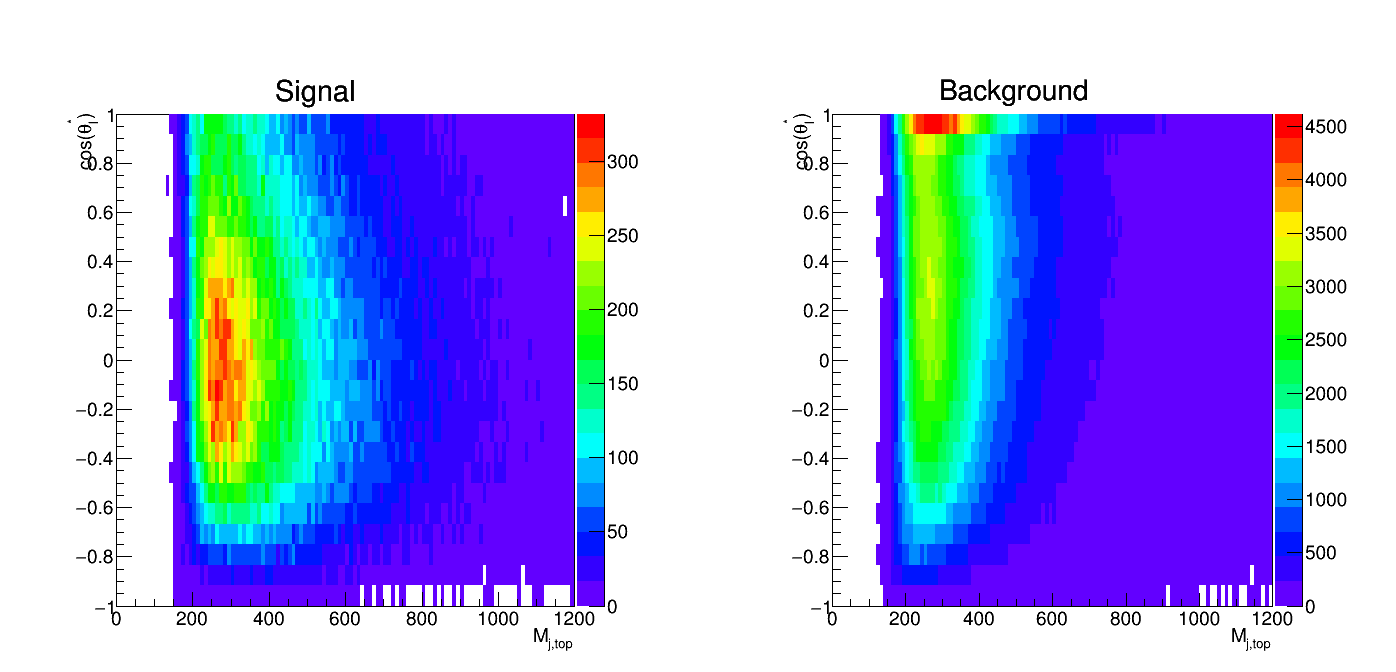
\includegraphics[width=0.9\textwidth]{/afs/ific.uv.es/user/p/pamarag/public/RedaccionTFM/Figuras/Correlation6x3/2d_signal_AND_bkg_PreSelTop_reco_tag_cos_S_Mjtop.png}
\caption{Two-dimensional distributions of $\cos(\theta_l^{*})$ versus $m_{j,top}$.}
\label{Fig:SB}
\end{figure}

%\begin{figure}[h]
%\centering
%\includegraphics[width=0.95\textwidth]%{/afs/ific.uv.es/user/p/pamarag/public/RedaccionTFM/Figuras/2d_signal_AND_bkg_tchannel_reco_tag_cos_S_kine_mlb_tag.png}
%\caption{wo-dimensional distributions of $\cos(\theta_l^{*})$ versus $m_{l,b}$.}
%\end{figure}


\clearpage


